\documentclass[aspectratio=169, 11pt]{beamer}

% --- Packages & Setup ---
\usepackage[utf8]{inputenc}
\usepackage[T1]{fontenc}
\usepackage{helvet}
\renewcommand{\familydefault}{\sfdefault}
\usepackage{xcolor}
\usepackage{booktabs}
\usepackage{graphicx}
\usepackage{tikz}
\usetikzlibrary{calc}

\graphicspath{{figures/}{../}{./}}

% --- Branding Colors ---
\definecolor{amritaMaroon}{HTML}{A4123F}

% --- Theme Setup ---
\usetheme{Madrid}
\usecolortheme[named=amritaMaroon]{structure}
\setbeamertemplate{navigation symbols}{}
\setbeamertemplate{footline}[frame number]

% Reduce block padding globally to prevent vertical overflow
\addtobeamertemplate{block begin}{\vspace*{-2pt}}{\vspace*{-2pt}}
\addtobeamertemplate{block end}{}{\vspace*{-4pt}}

\begin{document}

% =========================================================================
% TITLE SLIDE (Research-Based Project)
% =========================================================================
\begin{frame}
    \begin{tikzpicture}[remember picture,overlay]
        \node[fill=amritaMaroon, text=white, font=\bfseries\footnotesize, anchor=north east, rounded corners=2pt, inner sep=5pt]
        at ($(current page.north east) + (-0.2cm,-0.2cm)$)
        {Type 1: Research Project};
    \end{tikzpicture}

    \centering
    
\includegraphics[width=2.5cm]{logo.png}
    \vspace{0.05cm}

    {\large \textbf{\textcolor{amritaMaroon}{
    EvoSynth: Dynamic Multi-Armed Bandit Meta-Optimizer for\\
    Automated Model Selection and Hyperparameter Tuning
    }}} \\
    \vspace{0.05cm}
    {\footnotesize \textbf{23CSE498 -- Project Phase II (External Review)} \quad | \quad \textbf{Team Number: [2]}} \\
    \vspace{0.1cm}

    % Student Table
    \begin{table}
        \centering
        \footnotesize
        \renewcommand{\arraystretch}{1.05}
        \begin{tabular}{|c|c|l|}
            \hline
            \textbf{S.No} & \textbf{Register Number} & \textbf{Student Name} \\
            \hline
            1 & CB.SC.U4CSE23445 & Shivam Kharat \\
            \hline
            2 & CB.SC.U4CSE23565 & Siddharth Ladda \\
            \hline
            3 & CB.SC.U4CSE23627 & Kaushal Loya \\
            \hline
            4 & CB.SC.U4CSE23639 & Paarthu Reddy \\
            \hline
            5 & CB.SC.U4CSE23642 & Priyansh Narang \\
            \hline
        \end{tabular}
    \end{table}
    \vspace{0.05cm}

    {\footnotesize Guide: \textbf{Dr. Thangavelu S.}, Associate Professor, Department of CSE} \\
    {\scriptsize \today}
\end{frame}

% =========================================================================
% SLIDE 2: GUIDE APPROVAL EMAIL CONFIRMATION (Mandatory)
% =========================================================================
\begin{frame}{Guide Review \& Submission Approval}
    \framesubtitle{Confirmation of Project Review and Approval from Guide}
    \centering
    \begin{figure}
        \centering
        \includegraphics[
            width=0.80\textwidth,
            height=0.68\textheight,
            keepaspectratio
        ]{approval.png}
    \end{figure}
\end{frame}

% =========================================================================
% SECTION 1: PROBLEM DEFINITION, RESEARCH MOTIVATION & SOLUTION DESIGN
% =========================================================================
\section{Problem \& Solution Design}

% --- SLIDE 1: PROBLEM DEFINITION & RESEARCH MOTIVATION ---
\begin{frame}{1. Problem Definition \& Research Motivation}
    \framesubtitle{Problem Statement, Identified Literature Gap \& Objectives}

    \begin{block}{Problem Statement}
        \scriptsize
        \begin{itemize}
            \setlength{\itemsep}{1pt}
            \item \textbf{Core Problem:} Most tuners commit the whole budget to one search algorithm chosen in advance, yet the best algorithm differs from problem to problem and cannot be known beforehand.
            \item \textbf{Domain Context:} By the No Free Lunch theorem, no single optimizer dominates everywhere; budget should move online to whichever optimizer is making progress.
        \end{itemize}
    \end{block}

    \begin{block}{Existing Limitations \& Research Gap}
        \scriptsize
        \begin{itemize}
            \setlength{\itemsep}{1pt}
            \item \textbf{Existing Methods:} Optuna (one sampler per study), FLAML (cost-frugal local search), H2O (stacked ensembles); MaxUCB \cite{balef2025cash} (bandit over model classes, one tuner each); RL-DAS \cite{guo2024deep} (offline-trained switching among DE variants).
            \item \textbf{Research Gap:} No framework runs a portfolio of evolutionary optimizers concurrently on one CASH space, reallocates budget among them online without offline training, with swaps and rollback, and delivers a single model.
        \end{itemize}
    \end{block}

    \begin{block}{Research Objectives}
        \scriptsize
        \begin{itemize}
            \setlength{\itemsep}{1pt}
            \item \textbf{Objective 1:} UCB1 multi-armed bandit meta-engine routing budget among GA, PSO, DE and CMA-ES in real time.
            \item \textbf{Objective 2:} Live strategy switching (tier SWAPs with rollback) driven by improvement and diversity monitoring.
            \item \textbf{Objective 3:} Accuracy level with the strongest tuned baselines under an identical held-out protocol, from a single deployable model with measured inference cost.
        \end{itemize}
    \end{block}
\end{frame}

% --- SLIDE 2: PROPOSED METHODOLOGY & OVERALL WORKFLOW ---
\begin{frame}{2. Proposed Methodology \& Overall Workflow}
    \framesubtitle{End-to-End Research Methodology / System Workflow Architecture}
    \vspace{-0.35cm}
    % Full slide width (edge to edge minus 2 mm each side); keepaspectratio picks
    % whichever of width/height binds first, so the figure never overflows.
    \centering
    \makebox[\textwidth][c]{%
        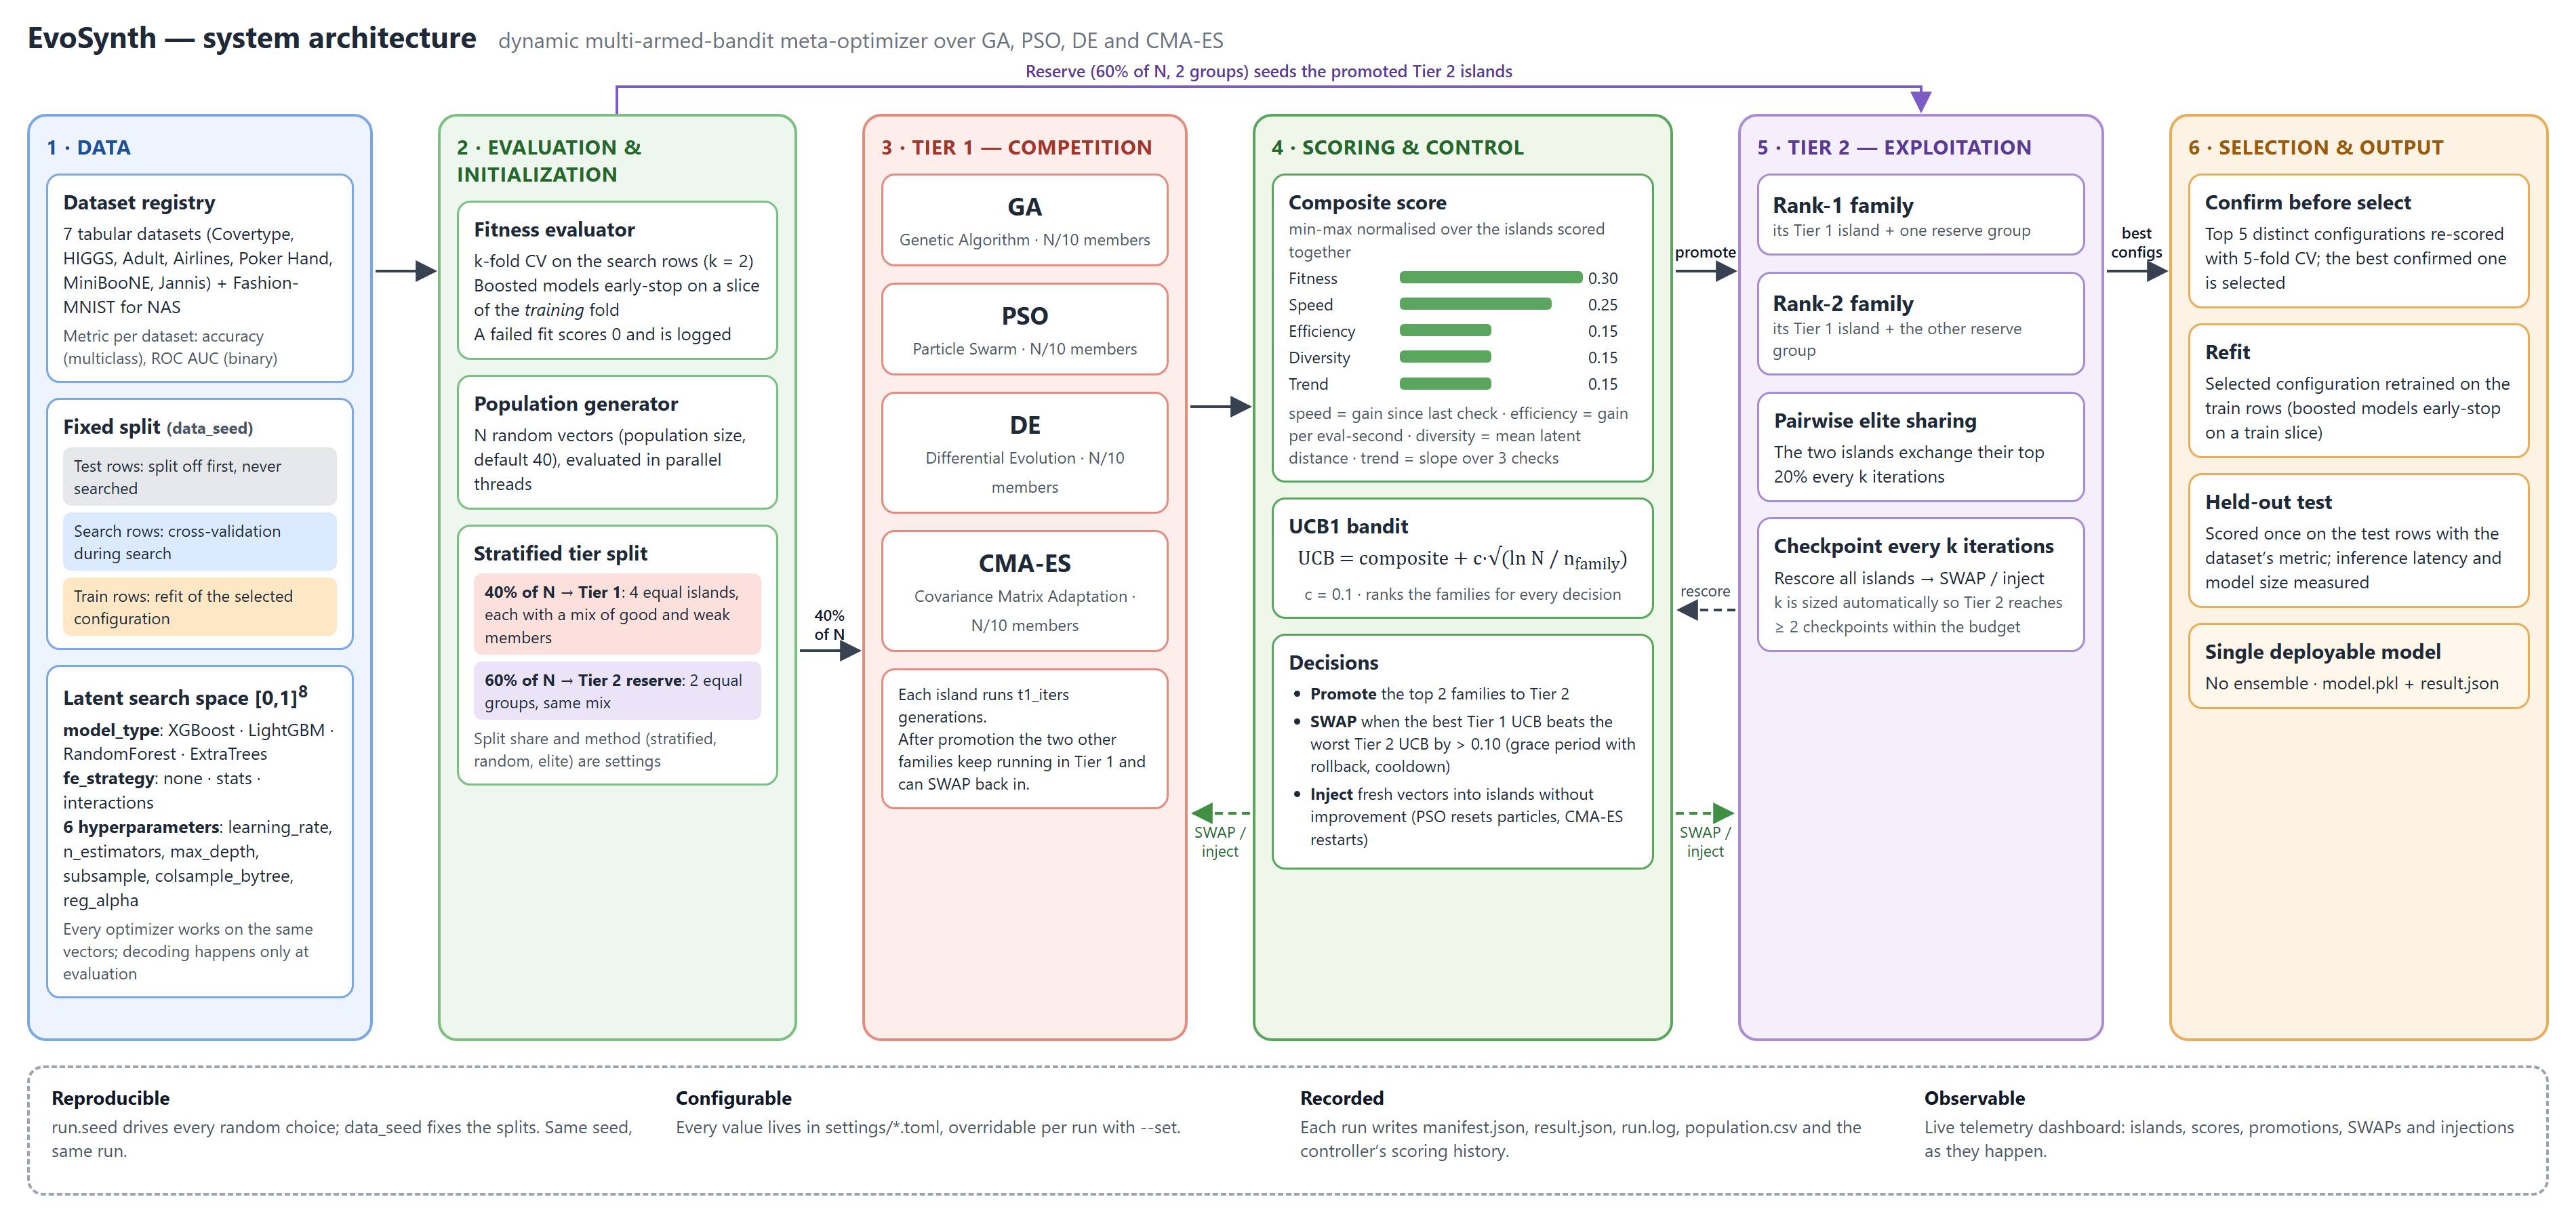
\includegraphics[
            width=\dimexpr\paperwidth-4mm\relax,
            height=0.8\textheight,
            keepaspectratio
        ]{arch.png}%
    }

    % \begin{block}{Workflow Summary}
    %     \scriptsize
    %     Encode search space to $[0,1]^d$ $\to$ stratified split: 40\% Tier-1 (4 islands of $N/10$: GA, PSO, DE, CMA-ES) $\to$ UCB1 promotes top-2 $\to$ 60\% reserve joins Tier-2, pairwise elite sharing, SWAP/rollback $\to$ confirm top-5 with 5-fold CV $\to$ one refit on train rows $\to$ single model scored once on held-out test rows.
    % \end{block}
\end{frame}

% --- SLIDE 3: METHODOLOGICAL COMPONENTS & FORMULATION ---
\begin{frame}{3. Methodological Components \& Formulation}
    \framesubtitle{Sub-Module Breakdown, Governing Mathematical Model \& Datasets}
    \begin{columns}[T]
        \column{0.49\textwidth}
        \begin{block}{Methodological Breakdown}
            \scriptsize
            \begin{itemize}
                \setlength{\itemsep}{1pt}
                \item \textbf{UCB1 Bandit Meta-Engine:} 5-metric composite rewards fitness, improvement, efficiency, diversity and trend.
                \item \textbf{Two-Tier Island Model:} stratified Tier-1 (40\%, 4 islands of $N/10$) competes 4 optimizers; top-2 promoted, each taking half of the 60\% reserve; pairwise elite sharing.
                \item \textbf{Stagnation Guard:} no improvement triggers random injection; live SWAP if a T1 algo's UCB exceeds the weaker T2 algo's by $>0.10$.
            \end{itemize}
        \end{block}

        \begin{block}{Mathematical Formulation}
            \scriptsize
            \begin{itemize}
                \setlength{\itemsep}{1pt}
                \item \textbf{UCB1 Formula:} $UCB_i = CS_i + c\sqrt{\frac{\ln(E_{\text{total}})}{E_i}}$ \ ($c=0.1$)
                \item \textbf{Composite:} $CS = 0.30F + 0.25S + 0.15E + 0.15D + 0.15T$ (min--max normalised)
                \item \textbf{Metrics:} $F$=Fit, $S$=Speed, $E$=Eff, $D$=Div, $T$=Trend
            \end{itemize}
        \end{block}

        \column{0.49\textwidth}
        \begin{block}{Dataset Specifications}
            \scriptsize
            \begin{itemize}
                \setlength{\itemsep}{1pt}
                \item \textbf{Covertype:} 581,012 samples, 54 features, 7 classes (accuracy). \textbf{Adult:} 48,842 samples, 14 features, binary (ROC AUC). 8 datasets supported.
                \item \textbf{Protocol:} test rows split off first (20k / 12k); search on 10k rows with 2-fold CV; top 5 confirmed with 5-fold CV; refit on train rows (60k / 36k). Exact splits on Zenodo.
                \item \textbf{Feature Engineering:} Generic Feature Engineer with searchable strategies: \texttt{none}, \texttt{stats}, \texttt{interactions}.
            \end{itemize}
        \end{block}

        \begin{block}{Evaluation Metrics}
            \scriptsize
            \begin{itemize}
                \setlength{\itemsep}{1pt}
                \item \textbf{Test score:} accuracy or ROC AUC on held-out rows, scored once.
                \item \textbf{Search wall time} and \textbf{inference cost} (ms/row, model MB).
                \item \textbf{Ablation:} each optimizer alone vs EvoSynth at equal budget.
            \end{itemize}
        \end{block}
    \end{columns}
\end{frame}

% =========================================================================
% SECTION 2: IMPLEMENTATION COMPLETION (100%)
% =========================================================================
\section{Implementation Details}

% --- SLIDE 4: IMPLEMENTATION COMPLETION (100%) - OVERVIEW ---
\begin{frame}{4. Implementation Details -- Overview}
    \framesubtitle{Module-Wise Implementation \& Pipeline Integration Status}
    \vspace{-0.15cm}
    \begin{table}
        \centering
        \tiny
        \renewcommand{\arraystretch}{1.1}
        \begin{tabular}{p{3.2cm} p{7.4cm} c}
            \toprule
            \textbf{Module / Stage} & \textbf{Implemented Functionality} & \textbf{Status} \\
            \midrule
            Latent Space Mapping & Mixed params encoded to $[0,1]^d$; categoricals binned by $\lfloor zK\rfloor$ & 100\% (Integrated) \\
            Meta-Engine (UCB1) & Composite scoring, UCB1 bonus, promotion, swap + rollback, decision log & 100\% (Integrated) \\
            Worker Optimizers & Ask/Tell wrappers for GA, PSO, DE, CMA-ES with state-aware injection & 100\% (Integrated) \\
            Tier Manager & Stratified 40/60 split, pairwise elite sharing, stagnation injection & 100\% (Integrated) \\
            Datasets \& Evaluators & 8 real datasets with fixed splits; XGBoost/LightGBM/RF/ExtraTrees + FE + early stopping; CNN for NAS & 100\% (Functional) \\
            Selection \& Refit & Confirm before select (top 5, 5-fold CV), shared refit, inference measurement & 100\% (Integrated) \\
            Experiment Harness & Baselines (Random, Optuna, FLAML, defaults), ablation, speed-up, resumable runner & 100\% (Integrated) \\
            Live Telemetry Dashboard & FastAPI SSE stream into React (Vite + Tailwind) & 100\% (Integrated) \\
            \bottomrule
        \end{tabular}
    \end{table}
    \vspace{-0.2cm}

    \begin{block}{Implementation Environment \& Repository}
        \scriptsize
        \begin{itemize}
            \setlength{\itemsep}{1pt}
            \item \textbf{Compute Environment:} Python 3.14, XGBoost, LightGBM, scikit-learn, PyTorch, Optuna, FLAML, React (12-thread laptop CPU, zero GPU).
            \item \textbf{Repository \& Deliverables:} \href{https://github.com/paarthureddy/EvoSynth}{\textcolor{blue}{GitHub}} \quad | \quad \href{https://evosynth-2027.github.io/evosynth-docs/}{\textcolor{blue}{Docs}} \quad | \quad \href{https://doi.org/10.5281/zenodo.23645119}{\textcolor{blue}{Zenodo Dataset (EvoSynth-Bench)}}
        \end{itemize}
    \end{block}
\end{frame}

% --- SLIDE 5: CORE MODULE IMPLEMENTATION DETAILS ---
\begin{frame}{5. Core Module Implementation Details}
    \framesubtitle{Two-Tier Control Logic, Parameter Configurations \& Interfaces}
    \begin{columns}[T]
        \column{0.52\textwidth}
        \begin{block}{Two-Tier Control Flow}
            \scriptsize
            \begin{itemize}
                \setlength{\itemsep}{1pt}
                \item \textbf{Init:} Population evaluated in parallel; stratified 40\% Tier-1 / 60\% reserve.
                \item \textbf{Tier-1 Tournament:} GA, PSO, DE, CMA-ES compete for $T_1$ iters.
                \item \textbf{Promotion:} Composite + UCB1 bonus ranks; top-2 move to Tier-2.
                \item \textbf{Live SWAP:} T1 algo replaces weaker T2 one if its UCB leads by $>0.10$.
                \item \textbf{Rollback:} Must beat global best within 5 iters, else reverted.
                \item \textbf{Elite Sharing:} The two T2 islands trade their top 20\% pairwise.
                \item \textbf{Output:} top 5 confirmed with 5-fold CV; one refit; one test score.
            \end{itemize}
        \end{block}

        \begin{block}{Generic Feature Engineer}
            \scriptsize
            \begin{itemize}
                \setlength{\itemsep}{1pt}
                \item \textbf{Searchable Gene:} \texttt{fe\_strategy} $\in$ \{\texttt{none}, \texttt{stats}, \texttt{interactions}\}.
                \item \textbf{Dataset-Agnostic:} No domain-specific column names; pure tabular math.
            \end{itemize}
        \end{block}

        \column{0.46\textwidth}
        \centering
        {\scriptsize \textbf{\textcolor{amritaMaroon}{Default Parameter Setup}}}
        \vspace{0.05cm}
        \begin{table}
            \centering
            \tiny
            \renewcommand{\arraystretch}{1.0}
            \begin{tabular}{lc}
                \toprule
                \textbf{Parameter} & \textbf{Value} \\
                \midrule
                Evaluation budget & 500 \\
                Population size & 40 \\
                Tier-1 / Tier-2 split & 40\% / 60\% \\
                Tier-1 iterations & 5 \\
                Checkpoint interval $k$ & 3 (auto) \\
                Exploration constant $c$ & 0.1 \\
                Swap margin (UCB) & 0.10 \\
                Rollback grace period & 5 iters \\
                Elite share & top 20\% \\
                Injection (T1 / T2) & 50\% / 20\% \\
                Search space dims & 8 (incl.\ model, FE) \\
                Model families & 4 (XGB, LGBM, RF, ET) \\
                Confirmation & top 5, 5-fold CV \\
                \bottomrule
            \end{tabular}
        \end{table}
    \end{columns}
\end{frame}

% =========================================================================
% SECTION 3: PRELIMINARY VERIFICATION & DEMONSTRATION
% =========================================================================
\section{Verification \& Demonstration}

% --- SLIDE 6: PRELIMINARY VERIFICATION & QUANTITATIVE RESULTS ---
\begin{frame}{6. Preliminary Verification \& Quantitative Results}
    \framesubtitle{Held-out test score, identical protocol, 500 evaluations, seed 42}
    \begin{table}
        \centering
        \scriptsize
        \renewcommand{\arraystretch}{1.15}
        \begin{tabular}{p{4.0cm} c c c c}
            \toprule
             & \multicolumn{2}{c}{\textbf{Covertype (accuracy)}} & \multicolumn{2}{c}{\textbf{Adult (ROC AUC)}} \\
            \textbf{Method / Configuration} & \textbf{Test} & \textbf{Time} & \textbf{Test} & \textbf{Time} \\
            \midrule
            Best Untuned Model & 89.77\% & -- & 92.92\% & -- \\
            FLAML (same wall time) & 92.53\% & 13.0\,m & \textbf{93.13\%} & 3.0\,m \\
            Random Search & \textbf{93.89\%} & 42.4\,m & 92.98\% & 19.1\,m \\
            Optuna TPE & 93.87\% & 49.8\,m & 92.95\% & 3.3\,m \\
            \midrule
            \textbf{EvoSynth} & \textbf{93.89\%} & \textbf{12.2\,m} & 92.96\% & \textbf{3.0\,m} \\
            \bottomrule
        \end{tabular}
    \end{table}
    \vspace{-0.15cm}

    \begin{block}{Experimental Verification Summary}
        \scriptsize
        \begin{itemize}
            \setlength{\itemsep}{1.5pt}
            \item \textbf{Quantitative Findings:} EvoSynth ties Random Search and Optuna (within 0.03) and picks the right model family per dataset (ExtraTrees + interactions on Covertype, XGBoost on Adult); fastest on Covertype through parallel evaluation (6.1$\times$ measured). Ablation: matches the best single optimizer (82.35\% CV) without knowing it in advance.
            \item \textbf{Verification of Core Hypothesis:} Covertype run --- DE + CMA-ES promoted; $T1\_GA$ (UCB 0.592) swapped in for $T2\_DE$ (UCB 0.369); rolled back after its 5-iteration grace period; CMA-ES found the winner.
        \end{itemize}
    \end{block}
\end{frame}

% --- SLIDE 7: EXPERIMENTAL VISUALIZATIONS & PROTOTYPE DEMONSTRATION ---
\begin{frame}{7. Comparison with Existing Frameworks \& Demonstration}
    \framesubtitle{Positioning EvoSynth against Optuna, FLAML, and H2O AutoML}

    \vspace{-0.25cm}
    \begin{table}
        \centering
        \tiny
        \setlength{\tabcolsep}{3.5pt}
        \renewcommand{\arraystretch}{1.1}
        \resizebox{\textwidth}{!}{%
        \begin{tabular}{p{2.3cm} p{2.6cm} p{2.5cm} p{2.7cm} p{3.2cm}}
            \toprule
            \textbf{Aspect} & \textbf{Optuna} & \textbf{FLAML} & \textbf{H2O AutoML} & \textbf{EvoSynth (Ours)} \\
            \midrule
            Search paradigm & Single Bayesian (TPE/CMA) & Cost-frugal local search & Random/Bayesian search & \textbf{UCB1 Multi-Armed Bandit} \\
            Search strategies & Fixed 1 sampler/study & Single greedy method & Sequential single trial & \textbf{4 concurrent (GA,PSO,DE,CMA)} \\
            Strategy switching & None (static sampler) & None & None & \textbf{Tier SWAPs (UCB margin 0.10) + rollback} \\
            Diversity protection & None & None & None & \textbf{Pop.\ Diversity in UCB1} \\
            Feature engineering & Manual & Limited heuristics & Fixed preprocessing & \textbf{Dataset-Agnostic Gene} \\
            Production output & Single model & Single model & Heavy 10-model stack & \textbf{Single model (cost of that model)} \\
            Measured test (Covertype) & 93.87\% & 92.53\% & -- & \textbf{93.89\%} \\
            \bottomrule
        \end{tabular}%
        }
    \end{table}
    \vspace{-0.2cm}

    \begin{block}{Demonstration Overview}
        \scriptsize
        \begin{itemize}
            \setlength{\itemsep}{1pt}
            \item \textbf{Single-Model Output:} serving cost is that of the chosen model, measured: 0.26\,ms / 0.4\,MB (Adult XGBoost) to 12.5\,ms / 470\,MB (Covertype ExtraTrees); no stacking overhead.
            \item \textbf{Live Demo:} \texttt{evosynth run --full --dataset adult} runs end-to-end with the real-time React dashboard displaying UCB1 scores, SWAPs \& rollbacks.
        \end{itemize}
    \end{block}
\end{frame}

% =========================================================================
% SECTION 4: TECHNICAL KNOWLEDGE & VIVA VOCE
% =========================================================================
\section{Technical Knowledge}

% --- SLIDE 8: TECHNICAL JUSTIFICATION, DESIGN TRADE-OFFS & INSIGHTS ---
\begin{frame}{8. Technical Justification, Design Trade-offs \& Insights}
    \framesubtitle{Methodological Rationale, Trade-offs \& Boundary Conditions}
    \begin{columns}[T]
        \column{0.49\textwidth}
        \begin{block}{1. Methodological Justification}
            \scriptsize
            \begin{itemize}
                \setlength{\itemsep}{1pt}
                \item No single optimizer wins everywhere (NFL); the best one changed between runs (PSO, CMA-ES, DE). UCB1 routes budget to the leader while the exploration bonus prevents early lock-in.
                \item Two-tier structure separates exploration (T1) from exploitation (T2), balancing the explore-exploit tradeoff.
            \end{itemize}
        \end{block}

        \begin{block}{2. Design \& Parameter Trade-offs}
            \scriptsize
            \begin{itemize}
                \setlength{\itemsep}{1pt}
                \item \textit{Latent Space:} Slight decode overhead, but enables continuous optimizers (PSO/CMA-ES) to tune categoricals.
                \item \textit{Parallel evaluation:} 6.1$\times$ on 12 threads (measured); early stopping adds little (1.17$\times$ alone).
                \item \textit{Offline Meta-Optimization:} Zero inference latency penalty.
            \end{itemize}
        \end{block}

        \column{0.49\textwidth}
        \begin{block}{3. Boundary Conditions \& Edge Cases}
            \scriptsize
            \begin{itemize}
                \setlength{\itemsep}{1pt}
                \item Rollback guard: Swapped-in algo must beat global best in 5 iters, else reverted.
                \item Stagnation rescue: injection of 50\% (T1) / 20\% (T2) random members.
                \item Confirm before select: top 5 re-scored with 5-fold CV against noisy 2-fold scores.
            \end{itemize}
        \end{block}

        \begin{block}{4. Limitations \& Future Scope}
            \scriptsize
            \begin{itemize}
                \setlength{\itemsep}{1pt}
                \item \textit{Current:} Ties (does not beat) strong baselines; FLAML best on Adult; one seed; Covertype space has a plateau every method reaches; single machine.
                \item \textit{Future Scope:} Multi-seed runs on HIGGS / Poker Hand; NGOpt and surrogate-benchmark comparison \cite{benjamins2025carps}; latency-aware objective; Ray workers.
            \end{itemize}
        \end{block}
    \end{columns}
\end{frame}


% =========================================================================
% REFERENCES & THANK YOU
% =========================================================================
\setbeamertemplate{bibliography item}{\insertbiblabel}

\section{References}

\begin{frame}[allowframebreaks]{References}
\fontsize{6.5}{8}\selectfont
\begin{thebibliography}{99}

\item[] \textbf{Research Papers}

\bibitem{guo2024deep} H. Guo \textit{et al.}, ``Deep reinforcement learning for dynamic algorithm selection: A proof-of-principle study on differential evolution,'' \textit{IEEE Trans. Syst., Man, Cybern.: Syst.}, vol. 54, no. 7, pp. 4247--4259, 2024.

\bibitem{franceschi2025hyperparameter} L. Franceschi \textit{et al.}, ``Hyperparameter optimization in machine learning,'' \textit{Foundations and Trends in Machine Learning}, vol. 18, no. 6, pp. 1054--1201, 2025.

\bibitem{alcobaca2026literature} E. Alcoba\c{c}a and A. C. P. L. F. de Carvalho, ``A literature review on automated machine learning,'' \textit{Artificial Intelligence Review}, vol. 59, art. no. 5, 2026.

\bibitem{crepinsek2025overcoming} M. \v{C}repin\v{s}ek, M. Mernik, M. Bekovi\'{c}, M. Pintari\v{c}, M. Moravec, and M. Ravber, ``Overcoming stagnation in metaheuristic algorithms with MsMA's adaptive meta-level partitioning,'' \textit{Mathematics}, vol. 13, no. 11, art. no. 1803, 2025.

\bibitem{ma2025toward} Z. Ma, H. Guo, Y.-J. Gong, J. Zhang, and K. C. Tan, ``Toward automated algorithm design: A survey and practical guide to meta-black-box-optimization,'' \textit{IEEE Trans. Evol. Comput.}, 2025, doi:10.1109/TEVC.2025.3568053.

\item[] \textbf{Conference Papers}

\bibitem{balef2025cash} A. Rezaei Balef, C. Vernade, and K. Eggensperger, ``Put CASH on bandits: A max K-armed problem for automated machine learning,'' in \textit{Advances in Neural Information Processing Systems}, vol. 38, 2025; arXiv:2505.05226.

\bibitem{schneider2025overtuning} L. Schneider, B. Bischl, and M. Feurer, ``Overtuning in hyperparameter optimization,'' in \textit{Proc. 4th Int. Conf. Automated Machine Learning (AutoML)}, 2025; arXiv:2506.19540.

\bibitem{nagler2024reshuffling} T. Nagler, L. Schneider, B. Bischl, and M. Feurer, ``Reshuffling resampling splits can improve generalization of hyperparameter optimization,'' in \textit{Advances in Neural Information Processing Systems}, vol. 37, 2024.

\bibitem{erickson2025tabarena} N. Erickson \textit{et al.}, ``TabArena: A living benchmark for machine learning on tabular data,'' in \textit{Advances in Neural Information Processing Systems (Datasets and Benchmarks Track)}, vol. 38, 2025; arXiv:2506.16791.

\item[] \textbf{Preprints}

\bibitem{benjamins2025carps} C. Benjamins \textit{et al.}, ``carps: A framework for comparing N hyperparameter optimizers on M benchmarks,'' arXiv:2506.06143, 2025.

\end{thebibliography}
\end{frame}

\begin{frame}
    \centering
    {\Huge \textbf{\textcolor{amritaMaroon}{Thank You}}} \\[0.4cm]
    {\large \textbf{Questions \& Viva Voce}}
\end{frame}

\end{document}
